\chapter{Support vector machines}
\label{cha:SVMs}

Support Vector Machines (SVM) are a very popular method for linear (and non-linear)
classification. They have some properties:
\begin{itemize}
	\item they are \textbf{large margin classifiers}: the separating hyperplane is
		setted withing the largest margin possible between classes

	\item the \textbf{support vector} are the training examples (also only a small
		subset), the decision boundary is identified on few support vectors

	\item the \textbf{large margin} properties are formally showed to imply some
		generalization properties

	\item can easily be extended to non-linear separation (also with \textit{kernel
		machines} \ref{cha:kernel_machines})
\end{itemize}

\section{Hyperplanes}
All the hyperplanes that can separate the two subsets in Figure \ref{fig:hyperplanesSVMs}
classify correctly every example. If I use a perceptron I could end up with
every of those planes, depending on the starting position.
\begin{figure}[H]
	\centering
	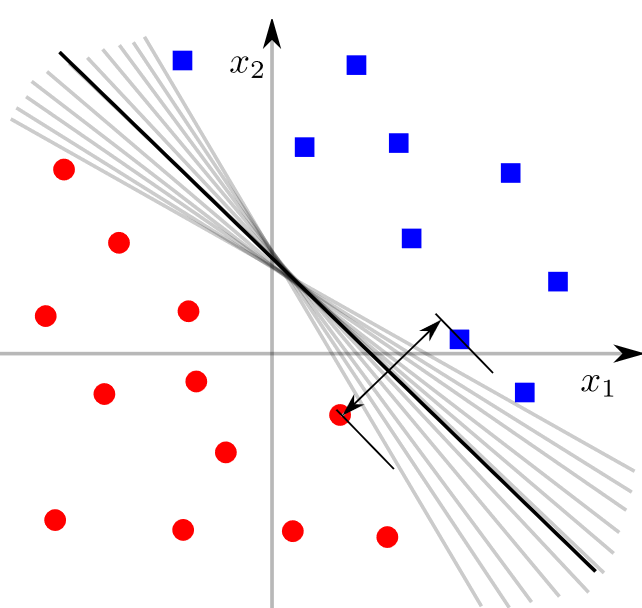
\includegraphics[scale=0.5]{
        images/13_SupportVectorMachines_hyperplanes.png
    }
	\caption{Possible hyperplanes separating two subsets}
	\label{fig:hyperplanesSVMs}
\end{figure}
SVMs learns the central hyperplane, the one that has the greater \textit{margin}.
The margin is the distance of the closest point to the hyperplane. SVM tries to
maximize this distance from both classes. This is intuitively a good choice:
leaves the most space between samples.

\defi{\textbf{Classifier margin}\label{def:classifier_margin}\\ Given a training set $\mathcal{D}$, a classifier confidence margin is \[\rho = min_{(\pmb{x}, y) \in \mathcal{D}}yf(\pmb{x})\] This is the minimal confidence of the classifier in a correct prediction (which corresponds to $yf(\pmb{x})$ as for perceptrons) and has to be positive in order to correctly separate the classes.\\ The \textit{geometric margin} is the same value divided by the norm of $\pmb{w}$: \[\frac{\rho}{||\pmb{w}||}= min_{(\pmb{x}, y) \in \mathcal{D}}\frac{yf(\pmb{x})}{||\pmb{w}||}\] }

\section{Hard margin SVMs}
We want intuitively learn a classifier that learns correct prediction with a
large margin. We need to fix degrees of freedom of hyperplanes in the space.
\defi{\textbf{Canonical hyperplane}\label{def:canonical_hyperplane}\\ There is a infinite number of equivalent hyperplanes that encode for the same hyperplane: \[\alpha(\pmb{w}^{T}\pmb{x}+ w_{0}) = 0\] for any $\alpha \neq 0$. The \textit{canonical hyperplane} is the hyperplane having the confidence (classifier margin \ref{def:classifier_margin}) equal to 1 \[\rho = min_{(\pmb{x}, y) \in \mathcal{D}}yf(\pmb{x}) = 1\] and its geometric margin is \[\frac{\rho}{||\pmb{w}||}= \frac{1}{||\pmb{w}||}\] }
We basically want to remove the degree of freedom because it would lead us to compute
for the same hyperplane multiple times. Therefore we will set $\rho = 1$ in
order to use only the canonical hyperplane. We can always do it until $\rho$ it is
not negative and provided that the samples are linearly separable.
\begin{figure}[H]
	\centering
	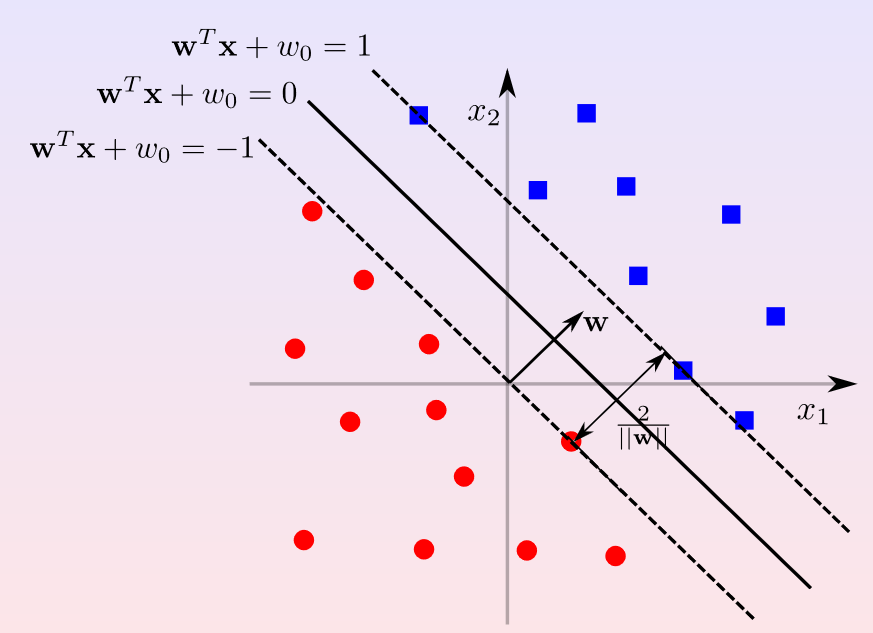
\includegraphics[scale=0.4]{
		images/13_SupportVectorMachines_canonicalHyperplane.png
	}
	\caption{Canonical hyperplane for each subsets}
	\label{fig:canonical_hyperplanes}
\end{figure}
As Figure \ref{fig:canonical_hyperplanes} shows, the dashed lines are the hyperplanes
for which the confidence margins are smallest and equal to 1 (and -1). They are the
hyperplanes with confidence 1 for class red (labelled as -1) and class blue (as +1).
Overall it always mean that $yf(x) = 1$ (taking into account the labels of the classes).
The geometric margin becomes $\frac{2}{||w||}$.

\theo{\textbf{Margin error bound (theorem)}\label{theo:margin_error_SVM}\\ Hard margin SVM Theorem (Margin Error Bound) Consider the set of decision functions $f(\mathbf{x})=\operatorname{sign}^{T}\mathbf{x}$ with $\|\mathbf{w}\| \leq \Lambda$ and $\|\mathbf{x}\| \leq R$, for some $R, \Lambda>0$. Moreover, let $\rho>0$ and $\nu$ denote the fraction of training examples with margin smaller than $\rho /\|\mathbf{w}\|$, referred to as the margin error. For all distributions $P$ generating the data, with probability at least $1-\delta$ over the drawing of the $m$ training patterns, and for any $\rho>0$ and $\delta \in(0,1)$, the probability that a test pattern drawn from $P$ will be misclassified is bound from above by \[\nu+\sqrt{\frac{c}{m}\left(\frac{R^2 \Lambda^2}{\rho^2}\ln^{2}m+\ln (1 / \delta)\right)}.\] \noindent Here, $c$ is a universal constant. Support Vector Machine }
\noindent
(you are not supposed to know the theorem by heart).\\ Basically, this theorem shows
a bound on the generalization error of a classifier which is trained to be a hard
margin SVM maximized. It happens that the generalization error (expected error)
for unseen example is a combination of:
\begin{enumerate}
	\item \textbf{sum of margins errors $\nu$} that stands for the component of
		all margin errors (training errors or examples with not enough confidence)

	\item \textbf{the second term} depends on number of training examples $m$ (the
		greater is $m$, the smaller is this factor) and $\rho^{2}$ which has to do with
		the margin (the larger the margin, the smaller the error)
\end{enumerate}

\textbf{Remark:} if $\rho$ is fixed to 1 (canonical hyperplane), maximizing
margin corresponds to minimizing $||\pmb{w}||$.

\subsection{Learning problem}
The learning objective of SVMs is indeed:
\begin{equation}
	min_{\pmb{w}, w_0}\frac{1}{2}||\pmb{w}||^{2}
\end{equation}
since when $\rho$ is fixed to 1 (canonical hyperplane), maximizing margin
corresponds to minimizing $||\pmb{w}||$. This is subject to
\[
	y_{i}(\pmb{w}^{T}\pmb{x}_{i}) + w_{0}\geq 1
\]
for all $(\pmb{x}_{i}, y_{i}) \in \mathcal{D}$. The hard margin is called this
way because it require all the example to have a confidence at least equal to 1.
Hard because it is not always possible. It there is no hyperplane that has this property,
the problem has no solution. Hard stands for the hard constraint, difficult to
obtain. This problem is a quadratic optimization problem (in $w$), with
quadratic objective so overall it is a quadratic optimization problem (reasonably
efficient with no local optima, but only one overall optima).\\ We could solve it
for standard tool for quadratic optimization, since it is a convex problem, it is
guaranteed that when we find a solution, is globally optimal.

\subsubsection{Techniques for solving the problem}
\textbf{Karush-Kuhn-Tucker approach (KKT)}\\ A constrained optimization problem
(of which I can minimize the objective but not guaranteeing that it satisfy the constraints)
can be addresses by converting it into an \textit{unconstrained} problem with the
same solution. Let's have a general constrainted optimization problem with
objective
\[
	min_{z}f(x)
\]
subject to (some constraint, in this case non-negativity constraints)
\[
	g_{i}(z) \geq 0 \quad \forall i
\]
Let's introduce a non-negative variable $\alpha_{i}\geq 0$ (called \textit{Lagrange
multiplier}) for each constraint and rewrite the optimization problem as
Lagrangian as putting constraint inside the objective in this way:
\[
	min_{z}max_{\alpha \geq 0}f(z) - \sum_{i}\alpha_{i}g_{i}(x)
\]
where $i$ are the possible constraints and $\alpha_{i}$ varies depending on the constraint.
Basically we remove the constraint by adding it into the objective. This problem
has $z$ parameter that we want to minimize and $\alpha s$. We want to minimize
$z$ and maximize with respect to $\alpha$ which has to be non-negative. \\ The optimal
solution(s) $x^{*}$ for this problem are also optimal solution for the original
constrained problem. $x^{*}$ will minimize the original problem and satisfy the constraints.\\

Suppose that we find $x'$, let's check whether it is an optimal solution if it does
\textbf{not} satisfy the constraints. If there is at least one constraint that $x
'$ does not satisfy, then there is some $i$ for which $g_{i}(z) < 0$ (it is negative).
If $g_{i}$ is negative, therefore the summation becomes positive and I can set
$\alpha$ to an infinite value. This leads to a non-valid solution for the original
problem.\\

Suppose now that $x'$ does satisfy all the constraints. Then the equivalent problem
formalized by KKT results in a finite number and therefore we know for sure that
the constraints are satisfied.\\ If we set all $\alpha s$ to zero, then the
summation goes to zero, therefore we have all constraint satisfied and also $z'$
will be a solution of $min_{z}f(z)$ (which is what we were looking for at the
beginning).\\

Applying the KKT approach to SVMs, then we can formalize out learning objective as:
\[
	min_{\pmb{w}, w_0}\frac{1}{2}||\pmb{w}||^{2}
\]
subject to:
\[
	y_{i}(\pmb{w}^{T}\pmb{x}_{i}+ w_{0}\geq 1)
\]
\[
	\forall (\pmb{x}_{i}, y_{i}) \in \mathcal{D}
\]
We now apply KKT and bring 1 to the other side.
\begin{equation}
	L(\pmb{w}, w_{0}, \alpha) = \frac{1}{2}||\pmb{w}||^{2}- \sum_{i=1}^{m}\alpha_{i}
	(y_{i}(\pmb{w}^{T}\pmb{x}_{i}+ w_{0}) - 1) \label{eq:Lagrangian}
\end{equation}
with L as \textit{Lagrangian} equivalent problem.\\ Again, $L$ gets minimized
with respect to \pmb{$w$}, $w_{0}$ and maximized from $\alpha_{i}$ (then we get the
solution for a saddle point).\\

We now try to solve the Lagrangian equivalent form. Let's take the gradient with
respect to $\pmb{w}, w_{0}$ and set it to zero.
\begin{align*}
	L                 & = \frac{1}{2}||\pmb{w}||^{2}- \sum_{i=1}^{m}\alpha_{i}(y_{i}(\pmb{w}^{T}\pmb{x}_{i}+ w_{0}) - 1)                                   \\
	\nabla_{\pmb{w}}L & = \nabla_{\pmb{w}}\left (\frac{\pmb{w}^{T}\pmb{w}}{2}\right) - \nabla_{\pmb{w}}\sum_{i=1}^{m}\alpha_{i}y_{i}\pmb{w}^{T}\pmb{x}_{i} \\
	                  & = \frac{2\pmb{w}}{2}- \sum_{i=1}^{m}\alpha_{i}y_{i}\pmb{x}_{i}                                                                     \\
	                  & =\pmb{w}- \sum_{i=1}^{m}\alpha_{i}y_{i}\pmb{x}_{i}= 0                                                                              \\
	\pmb{w}           & = \sum_{i=1}^{m}\alpha_{i}y_{i}\pmb{x}_{i}
\end{align*}

\textbf{Remark:}
\[
	\nabla_{\pmb{w}}\sum_{i=1}^{m}\alpha_{i}(y_{i}(\pmb{w}^{T}\pmb{x}_{i}+ w_{0}) -
	1) = \nabla_{\pmb{w}}\sum_{i=1}^{m}\alpha_{i}y_{i}\pmb{w}^{T}\pmb{x}_{i}
\]
because $\alpha_{i}y_{i}\pmb{w}^{T}\pmb{x}_{i}$ is the only term which depends on
$\pmb{w}$. \\

Now we get
\begin{equation}
	\pmb{w}= \sum_{i=1}^{m}\alpha_{i}y_{i}\pmb{x}_{i}\label{ref:important_intermediate_result}
\end{equation}
defined in terms of alphas, but this is a way to write primal variables in terms
of secondary (dual) variables (the $\alpha$s). Let's also take the derivative of
the Lagrangian formulation with respect to $w_{0}$

\begin{align*}
	L            & = \frac{1}{2}||\pmb{w}||^{2}- \sum_{i=1}^{m}\alpha_{i}(y_{i}(\pmb{w}^{T}\pmb{x}_{i}+ w_{0}) - 1) \\
	\pdv{L}{w_0} & = \pdv{(- \sum_{i=1}^m \alpha_i y_i w_0)}{w_0}                                                   \\
\end{align*}

\textbf{Remark:} also in this case we take into account only the terms where $w_{0}$
appears.
\newline

Since it is linear, it becomes
\begin{equation}
	\sum_{i=1}^{m}\alpha_{i}y_{i}= 0 \label{ref:second important result}
\end{equation}

What we can do, is replacing $\pmb{w}$ with the formulation in terms of alphas ($w
= \sum_{i=1}^{m}\alpha_{i}y_{i}\pmb{x}_{i}$), getting

\begin{align*}
	L & = \frac{\pmb{w}^{T}\pmb{w}}{2}- \sum_{i=1}^{m}\alpha_{i}(y_{i}(\pmb{w}^{T}\pmb{x}_{i}+ w_{0}) - 1)                                                                                                                                                                 \\
	  & = \frac{1}{2}\left( \sum_{i=1}^{m}\alpha_{i}y_{i}\pmb{x}_{i}\right)^{T}{\sum_{j=1}^m \alpha_j y_j \pmb{x}_j}- \sum_{i=1}^{m}\alpha_{i}y_{i}(\sum_{j=1}^{m}\alpha_{j}y_{j}\pmb{x}_{j})^{T}\pmb{x}_{i}- \sum_{i=1}^{m}\alpha_{i}y_{i}w_{0}+ \sum_{i=1}^{m}\alpha_{i} \\
\end{align*}

Considering the first term, $\alpha, y$ are scalars (their transpose is still a scalar)
only $\pmb{x_i}, \pmb{x_j}$ are vectors. We compute the product excluding the scalar
part, therefore

\[
	L = \frac{1}{2}\sum_{i}\sum_{j}\alpha_{i}\alpha_{j}y_{i}y_{j}x_{i}^{T}x_{j}\dots
\]

But the second term
$-\sum_{i=1}^{m}\alpha_{i}y_{i}(\sum_{i=j}^{m}\alpha_{j}y_{j}\pmb{x}_{j})^{T}\pmb
{x}_{i}$
it is actually twice the quantity described by the first term. In the third term,
we get that $w_{0}$ does not depend on $i$, we can take it outside. At this
point we get:

\[
	L = \frac{1}{2}\sum_{i}\sum_{j}\alpha_{i}\alpha_{j}y_{i}y_{j}\pmb{x_i}^{T}\pmb{x_j}
	- \sum_{i}\sum_{j}\alpha_{i}\alpha_{j}y_{i}y_{j}\pmb{x_i}^{T}\pmb{x_j}- w_{0}\sum
	_{i=1}^{m}\alpha_{i}y_{i}+ \sum_{i=1}^{m}\alpha_{i}
\]

Since we defined $\pmb{w}= \sum_{i=1}^{m}\alpha_{i}y_{i}\pmb{x}_{i}$ (\ref{ref:important_intermediate_result}),
and also $\sum_{i=1}^{m}\alpha_{i}y_{i}= 0$ \ref{ref:second important result}, therefore
our objective becomes:

\[
	L(\alpha) = \sum_{i=1}^{m}\alpha_{i}- \frac{1}{2}\sum_{i}\sum_{j}\alpha_{i}\alpha
	_{j}y_{i}y_{j}\pmb{x_i}^{T}\pmb{x_j}
\]

Which is the final formulation for the Lagrangian. This has to be minimized with
respect to $\pmb{w}, w_{0}$ and maximized with respect to $\alpha$. We did get
rid of the minimization, we are now going to maximize with respect to $\alpha$.\\

Our objective becomes:
\[
	max_{\alpha \in \mathbb{R}^m}\sum_{i=1}^{m}\alpha_{i}- \frac{1}{2}\sum_{i}\sum_{j}
	\alpha_{i}\alpha_{j}y_{i}y_{j}\pmb{x_i}^{T}\pmb{x_j}
\]
and our constraints:
\[
	\alpha_{i}\geq 0 \quad i = 1, \dots, m
\]
\[
	\sum_{i=1}^{m}\alpha_{i}y_{i}= 0
\]
This is a dual formulation ($\alpha s$ are in this case the dual variables,
because they did not appear in the original problem but introduced in the
Lagrangian), while the original formulation was only in terms of the primal
variables. So we can formulate the constrained optimization problem in two ways (as
primal or dual), there forms are mediated via the Lagrangian. This is still a quadratic
optimization problem, the constraints are simpler then in the primal problem: we
had linear constraints which were not easy to keep updated. In the dual problem
we have easier constraint (non-negativity and bounding box constraint). The dual
formulation is easier to deal with. Overall there are many ways in which we can
solve it. Depending on the number of feature and number of samples (alphas
depend on $m$ number of examples, and $\pmb{w}$ depends on number of features $d$)
we can address this problem more easily from the primal or from the dual. \\

%If we solve for it we find the $\alpha s$, but eventually we need $\pmb{w}, w_0$.
We can write $f(\pmb{x})$ (the decision function) in term of the primal or the
dual (remember \ref{ref:important_intermediate_result})

\[
	f(\pmb{x}) = \pmb{w}^{T}\pmb{x}+ w_{0}= \sum_{i=1}^{m}\alpha_{i}y_{i}\pmb{x}_{i}
	^{T}\pmb{x}+ w_{0}
\]

\textbf{Why do we call this method \textit{support vector}?}\\ By the KKT
conditions, we get a Lagrangian and the Lagrangian multipliers ($\alpha s$). The
Lagrangian \ref{eq:Lagrangian} contains a combination that stand for the margin
(the inverse of the margin) and the constraints with Lagrangian multipliers. This
is a min-max problem (minimize wrt $\pmb{w}$ and maximize wrt $\alpha$s), the results
is a \textit{saddle point}. What we know is that at this point (optimum), each
of the conditions (constraint) should be equal to zero, therefore each element in
the summation should be zero. This happens in two ways:
\begin{enumerate}
	\item $\alpha_{i}$ are equal to zero, which means that the example $x_{i}$
		does not contribute to the final solution.

	\item $y_{i}(\pmb{w}^{T}\pmb{x}_{i}+ w_{0}) - 1 = 0$ (the other component of
		the product is equal to zero), which means that
		$y_{i}(\pmb{w}^{T}\pmb{x}_{i}+ w_{0}) = 1$. This means that the confidence for
		the examples should be one. There are two hyperplanes with confidence equal
		to one (positive and negative \ref{fig:canonical_hyperplanes}) but both
		satisfy this condition (\textbf{positive examples} with confidence $+1$ and
		\textbf{negative examples} with confidence $-1$). These are the only points (with
		exact confidence $=+1$ or $=-1$) with $\alpha_{i}> 0$ and these are the \textbf{support
		vectors} (SV).
\end{enumerate}
My decision hyperplane $f(x) = 0$ is defined only in terms of the support vectors.
All other points do not contribute in defining the decision function. This mean that
if I remove every other example from the training set (leaving only the support
vectors) I would get the very same classifier. SVMs are \textit{sparse}, this
means that only few of the training example will end up in SV. In many cases the
number of SV become much less than the training examples.\\

If we look at $f(\pmb{x})$ (which is the decision on x), is basically taken as a
linear combination of dot products between training data and $\pmb{x}$ this value
is high if the two values are similar. If $\pmb{x_i}$ is similar to $\pmb{x}$, the
high value will be multiplied by $y_{i}$ (class of $\pmb{x_i}$) and $\alpha_{i}$.
Basically each train example pulls towards its own class based on how similar
the new example is to him and proportionally to $\alpha_{i}$ (as weight). This prediction
is therefore performed on weighted similarity.\\

We previously calculated $\pmb{w}$ but we still need to compute $w_{0}$. I can use
the condition $y_{i}(\pmb{w}^{T}\pmb{x}_{i}+ w_{0}) = 1$ considering cases in which
$\alpha_{i}> 0$. Therefore the bias $w_{0}$ is:
\begin{align*}
	y_{i}(\pmb{w}^{T}\pmb{x}_{i}+ w_{0})                & = 1 \\
	y_{i}\pmb{w}^{T}\pmb{x}_{i}+ y_{i}w_{0}             & = 1 \\
	w_{0}= \frac{1 - y_{i}\pmb{w}^{T}\pmb{x}_{i}}{y_{i}}
\end{align*}
For each of the samples, we get a different $w_{0}$, therefore, out final value
will be their average.

\section{Soft margin SVMs}
There is one big problem with hard margin SVMs.
\begin{figure}[H]
	\centering
	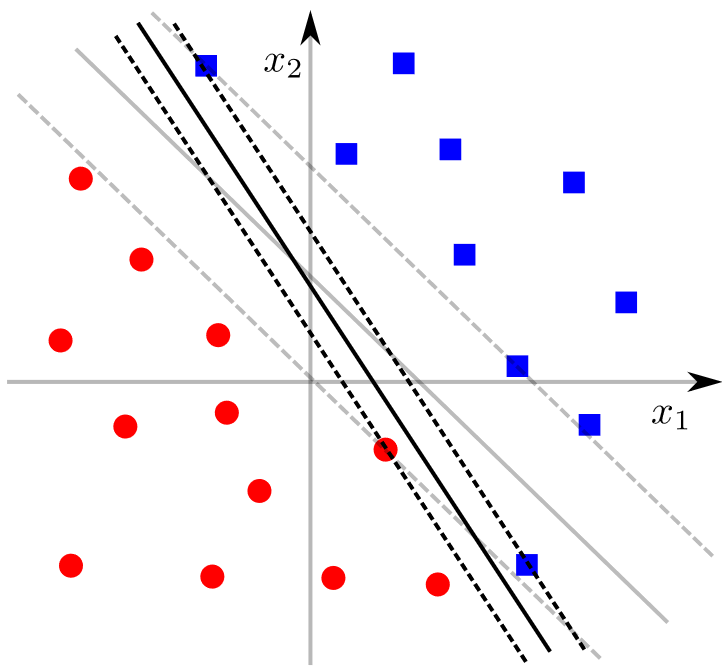
\includegraphics[scale=0.3]{
        images/13_SupportVectorMachines_hardSVM.png
    }
	\caption{By adding an additional blue point, the previous hyperplane is no longer
	a valid solution, by computing it again we get the black new hyperplane}
	\label{fig:hardSVM_problem}
\end{figure}
By adding an additional blue point as shown in Figure \ref{fig:hardSVM_problem},
the previous hyperplane is no longer a valid solution, by computing it again we get
the black new hyperplane which has a significantly smaller confidence and it is tilted.
Is it worth it? We should not assume that all labels are correct, we are maybe
\textbf{overfitting} training examples. A solution is using \textbf{soft margin}
SVMs.\\

We want to maximize the margin but with a soft constraint: some exceptions of falsely
classified samples are allowed. This intuition can be formalized as minimizing
the inverse of the margin subject to all examples being predicted in the correct
class with a confidence at least one, \textbf{but} we add a slack variable
$\xi_{i}$ for each sample in the dataset, then we will sum them up according to a
multiplicative factor C which is a hyperparameter.
\[
	min_{\pmb{w} \in \mathcal{X}, w_0 \in \mathbb{R}, \xi \in \mathbb{R}^m}\frac{||\pmb{w}||^{2}}{2}
	+ C\sum_{i=1}^{m}\xi_{i}
\]
subject to:
\begin{align*}
	y_{i}(\pmb{w}^{T}\pmb{x}_{i}+ w_{0}) & \geq 1 - \xi_{i}\quad i = 1, \dots, m \\
	\xi_{i}                              & \geq 0 \quad i = 1, \dots, m
\end{align*}
$- \xi_{i}$ the slack is measuring how far we are from satisfying the constraint:
\begin{itemize}
	\item if it is equal to zero we are correctly classifying the example

	\item if it is greater than zero we are miss-classifying that example

	\item the larger is $\sum_{i=1}^{m}\xi_{i}$, the larger is the number of miss-classified
		examples
\end{itemize}
By collecting all the slack variables $C\sum_{i=1}^{m}\xi_{i}$ (sum of penalties)
we are trying to combine margin maximization and penalty minimization. The summation
is weighted based on $C$ a regularization parameter constant greater than zero,
that gives a trade off between maximizing the margin and fitting the examples. If
$C = \infty$ we will have to correctly predict every example (we are back to
hard margins SVMs). The smaller the $C$, the more exception we allow.\\

The idea is that in this objective we are combining a large margin and having
few exception to the rule of large margin separation. Of course they are conflicting
objectives. There is a more general theory under this concept: \textbf{regularization
theory}. In regularization theory we have objectives to be learned that combine a
\textbf{complexity term} (in this case the norm of the weight vectors, the
margin but in general is a complexity of the solution) and \textbf{training
errors} (in term of a loss function, measure of the error is the case of SVMs).
\[
	min_{\pmb{w} \in \mathcal{X}, w_0 \in \mathbb{R}, \xi \in \mathbb{R}^m}\frac{||\pmb{w}||^{2}}{2}
	+ C\sum_{i=1}^{m}loss(y_{i}, f(\pmb{x}_{i}))
\]

In soft margin SVMs, then we need to specify what is the loss function
$loss(y_{i}, f(\pmb{x}_{i}))$. Basically $\xi_{i}$ is the loss of false predictions
\[
	\xi_{i}= loss(y_{i}, f(\pmb{x}_{i}))
\]
considering the constraint
\[
	y_{i}(\pmb{w}^{T}\pmb{x}_{j}+ w_{0}) \geq 1 - \xi_{i}
\]
\[
	y_{i}f(\pmb{x}_{i}) \geq 1 - \xi_{i}
\]
therefore
\[
	\xi_{i}\geq 1 - y_{i}(\pmb{w}^{T}\pmb{x}_{i}+ w_{0})
\]
remember also that $\xi$ is non-negative, so if we combine these things
basically we get that
\begin{equation}
	loss(y_{i}, f(\pmb{x}_{i})) = |1 - y_{i}f(\pmb{x}_{i})|_{+}= |1 - y_{i}(\pmb{w}
	^{T}\pmb{x}_{j}+ w_{0})|_{+}
\end{equation}

where $|\dots|_{+}$ stands for the value itself if it is positive and zero otherwise.
If we look at this loss function graphically we can plot it in terms of
$y f(\pmb{x})$
\begin{figure}[H]
	\centering
	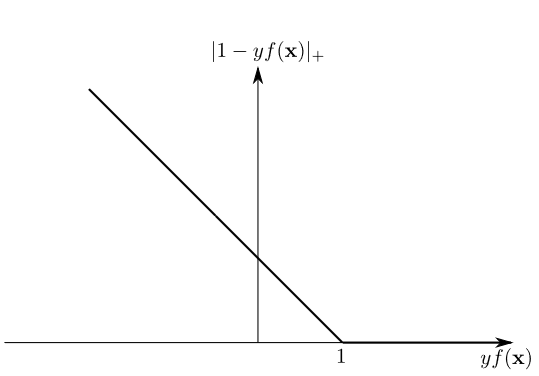
\includegraphics[scale=0.5]{
        images/13_SupportVectorMachines_hingeLoss.png
    }
	\caption{Plotting loss function (hinge loss)}
	\label{fig:plot_loss_fun}
\end{figure}
the loss function is zero if the confidence in the correct prediction is at
least one. If the confidence is less than one, then it is
$|1 - y_{i}f(\pmb{x}_{i})|_{+}$.\\ This loss function is called \textbf{hinge
loss function} since it is not a smooth loss function. It also shows why SVMs
are sparse: the loss function is zero in a part of a space helps having a sparse
solution (means that you don't care about differences, so the complexity term will
dominate). Still, this loss function can be minimized.

\subsection{Lagrangian for soft margin SVMs}
Let's compute the same calculation described before also for soft margin SVMs. Our
KKT formulation will be
\[
	L = \frac{1}{2}||\pmb{w}||^{2}+ C \sum_{i=0}^{m}\xi_{i}- \sum_{i=1}^{m}\alpha_{i}
	(y_{i}(\pmb{w}^{T}\pmb{x}_{i}+ w_{0}) - 1 + \xi_{i}) -\sum_{i=0}^{m}\beta_{i}\xi
	_{i}
\]

where $\sum_{i=0}^{m}\beta_{i}\xi_{i}$ are the Lagrangian multipliers for the
constraints $\xi_{i}\geq 0$. In this case, the primal variable are again
$\pmb{w}, w_{0}$, while the dual are $\alpha, \beta$. Let's now compute the
gradient of the Lagrangian
\begin{align*}
	\nabla_{\pmb{w}}L & = \nabla_{\pmb{w}}{\frac{1}{2} ||\pmb{w}||^2 + C \sum_{i=0}^m \xi_i - \sum_{i=1}^m \alpha_i (y_i (\pmb{w}^T \pmb{x}_i + w_0) - 1 + \xi_i) -\sum_{i=0}^m \beta_i \xi_i} \\
	                  & = \nabla_{\pmb{w}}\left( \frac{\pmb{w}^{T}\pmb{w}}{2}- \sum_{i=1}^{m}\alpha_{i}y_{i}\pmb{w}^{T}\pmb{x}_{i}\right)                                                      \\
	                  & = \pmb{w}- \sum_{i=1}^{m}\alpha_{i}y_{i}x_{i}
\end{align*}

therefore it does not change from hard margin
\begin{equation}
	\pmb{w}= \sum_{i=1}^{m}\alpha_{i}y_{i}x_{i}\label{eq:soft_margin_w_result}
\end{equation}
Then, we compute the derivative wrt $w_{0}$, but again does not change, since
there is only one term containing $w_{0}$, then zeroing it we get.
\begin{equation}
	\sum_{i=1}^{m}\alpha_{i}y_{i}= 0 \label{eq:soft_margin_w_0_result}
\end{equation}

Then, we need to compute also for slack variables. Here we compute gradients wrt
each of the $\xi_{i}$

\[
	\pdv{L}{\xi_i}= \pdv{}{\xi_i}(C\xi_{i}- \alpha_{i}\xi_{i}- \beta_{i}\xi_{i})
\]

By zeroing we get
\begin{equation}
	c - \alpha_{i}- \beta_{i}= 0 \label{eq:soft_margin_xi_gradient}
\end{equation}

If we replace this result \ref{eq:soft_margin_xi_gradient} in the Lagrangian (missing
calculations), for $\pmb{w}$ we get simplified results:
\[
	L(\alpha) = -\frac{1}{2}\sum_{i}\sum_{j}\alpha_{i}\alpha_{j}y_{i}y_{j}\pmb{x}_{i}
	^{T}\pmb{x}_{j}+ \sum \alpha_{i}
\]
that fully correspond exactly to the hard margin case. Therefore the dual formulation
is:
\begin{equation}
	max_{\alpha_{i=1}^m \in \mathbb{R}^m}\sum_{i=1}^{m}\alpha_{i}- \frac{1}{2}\sum_{i,
	j = 1}^{m}\alpha_{i}\alpha_{j}y_{i}y_{j}\pmb{x}_{i}^{T}\pmb{x}_{j}\label{eq:dual_formulation_object_soft}
\end{equation}
subject to
\[
	0 \leq \alpha_{i}\leq C \quad i = 1, \dots, m
\]
\[
	\sum_{i=1}^{m}\alpha_{i}y_{i}= 0
\]
In this soft constraint, $\alpha_{i}$ needs to be non-negative, but also at most
equal $C$ (from \ref{eq:soft_margin_xi_gradient}). This box constraint is the only
difference from the hard case when we transform the problem in the dual form.\\

The interesting fact is that the support vectors: in the Lagrangian (KKT
conditions), when we get to the saddle point it holds that
\[
	\alpha_{i}(y_{i}(\pmb{w}^{T}\pmb{x}_{i}+ w_{0}) - 1 + \xi_{i}) = 0 \quad \forall
	i
\]
and
\[
	\beta_{i}\xi_{i}= 0 \quad \forall i
\]
This implies that the support vectors, if $\alpha_{i}= 0$, the example does not
contribute to the decision. If $\alpha_{i}> 0$ than it is necessarily true that $(
y_{i}(\pmb{w}^{T}\pmb{x}_{i}+ w_{0}) - 1 + \xi_{i}) = 0$. This happens because
we have and additional constraint (\ref{eq:soft_margin_xi_gradient}) that is not
a KKT condition but comes directly from the derivative. Suppose that $\alpha_{i}<
C$, then
\[
	C - \alpha_{i}- \beta_{i}= 0 \implies \beta_{i}> 0
\]
If $\beta_{i}> 0$, then to satisfy $\beta_{i}\xi_{i}= 0$ we need $\xi_{i}= 0$.
Therefore
\[
	y_{i}(\pmb{w}^{T}\pmb{x}_{i}+ w_{0}) = 1
\]
which is the same condition of the hard margin SVMs. The examples stay on the hyperplane
with confidence one. For any example that has a confidence greater than zero but
smaller than $C$, this example stays on the hyperplane with confidence equal to one.
\\

For the examples for which $\alpha_{i}= C$, it means that $\beta_{i}= 0$, then $\xi
_{i}$ does not have to be equal to zero (typically it is not). Therefore the
example won't be on the confidence one hyperplane, but closer to the decision hyperplane
(the confidence is less than one). These are called \textit{margin errors}.\\
\begin{figure}[H]
	\centering
	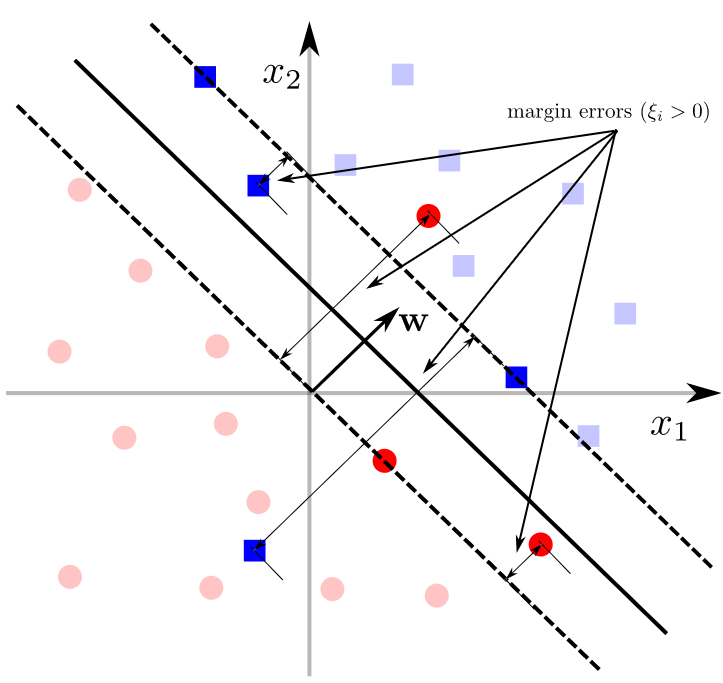
\includegraphics[scale=0.35]{
        images/13_SupportVectorMachines_softSVM.png
    }
	\caption{soft margin SVM with decision hyperplane, hyperplanes with confidence
	equal to one, bounded (on the hyperplanes) and unbounded support vectors (miss-labelled
	that training and margin errors or closer to the decision hyperplane that are margin
	error)}
	\label{fig:SVM_soft}
\end{figure}

Both the examples with $\alpha_{i}\leq 0$ belong to the so called \textit{support
vector} because they contribute to the definition of the separation hyperplane (bound
and unbound support vectors). All other having $\alpha_{i}> 0$ do not contribute
to the decision hyperplane.

\section{Large scale SVM learning}
Training SVMs is not very efficient (it is more than quadratic problem) for
large dataset. If we consider millions of example, SVMs training is not
something feasible. People have developed also procedures for large-scale SVMs which
is a stochastic gradient descent (GD).\\

The objective for SVMs is the following minimization
\[
	min_{\pmb{w} \in \mathcal{X}}\frac{\lambda}{2}||\pmb{w}||^{2}+ \frac{1}{m}|1 -
	y_{i}\langle \pmb{w}, \pmb{x}_{i}\rangle|_{+}
\]
where
\begin{itemize}
	\item the notation $\langle \dots \rangle$ stands for a dot product.

	\item in addition, $C = \frac{1}{m}$ for a large scale problem, since the training
		error could dominate. We normalize by the number of examples.

	\item $\lambda = \frac{1}{C}$

	\item there is no $w_{0}$, since with high dimensional problem this would mean
		preventing passing through the origin (not needed)

	\item we perform feature augmenting via adding $1$ in the sum.
\end{itemize}
Performing stochastic GD means that we compute gradient on single examples (not all
together). Therefore we are only considering $x_{i}y_{i}$

\[
	E(\pmb{w}, (\pmb{x}_{i}, y_{i})) = \frac{\lambda}{2}||\pmb{w}||^{2}+ |1 - y_{i}
	\langle \pmb{w}, \pmb{x}_{i}\rangle|_{+}
\]

This is the error only on \textbf{one} example. By computing the gradient on the
error

\[
	\nabla_{\pmb{w}}E(\pmb{w}, (\pmb{x}_{i}, y_{i})) = \lambda \pmb{w}+ \mathbb{1}[
	y_{i}\langle \pmb{w}, \pmb{x}_{i}\rangle < 1] y_{i}\pmb{x}_{i}
\]

At this point we do not know how to carry on, so we will compute a \textbf{subgradient}.
Whenever we do not have a single gradient in a point, we can perform a subgradient.
Its indicator function will be
\[
	\mathbb{1}[y_{i}\langle \pmb{w}, \pmb{x}_{i}\rangle < 1] =
	\begin{cases}
		1 & \text{if }y_{i}\langle \pmb{w}, \pmb{x}_{i}\rangle < 1 \\
		0 & \text{otherwise}
	\end{cases}
\]
The subgradient of a function $f$ in a point $\pmb{x}_{0}$ is any vector
$\pmb{v}$ such that for any $\pmb{x}$ hold the condition:
\[
	f(\pmb{x}) - f(\pmb{x}_{0}) \geq \pmb{v}^{T}(\pmb{x}- \pmb{x}_{0})
\]
This means that when we have discontinuity for the derivative (gradient) we could
find subgradients.
\begin{figure}[H]
	\centering
	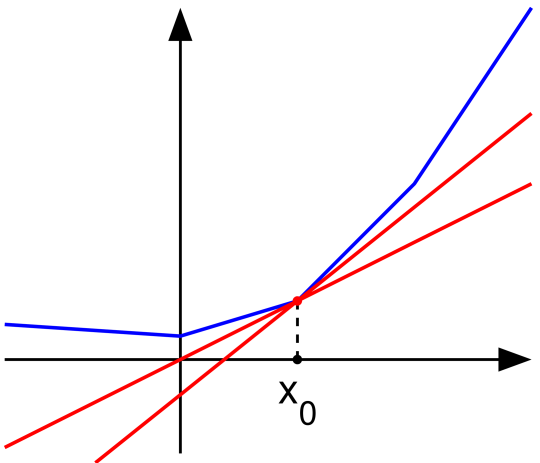
\includegraphics[scale=0.3]{
        images/13_SupportVectorMachines_subgradient.png
    }
	\caption{Visual representation of a subgradient for a point $x_{0}$, the voice
	of $\pmb{v}$ is among the red lines}
	\label{fig:subgradient}
\end{figure}
We could use any of the (red) vectors that satisfy the condition. The selection of
$\pmb{v}$ is defined by the indicator function that tells me if the confidence is
smaller than one. We then can get the exact gradient in each point and then
perform subgradient descent.

This means that we update along with the error rate. The only additional piece,
is that the learning rate is not constant, but decreases with $\lambda = \frac{1}{C}$
and on $t$, which is pretty common in GD. This has some theoretical guarantees,
but there is no need for theoretical details.\\